% !TeX root = ../main.tex

\chapter{关于第三章的一些补充材料}

\section{两个缝合矩阵以及Pfaffian的一些性质}\label{cbrelation1}

对于式\eqref{sewingm}定义的缝合矩阵$B$,
我们可以直接求出它的矩阵元如下,
\begin{equation}
	\begin{split}\label{smb}
	\quad \krin{u_m(-\vb k),\mathcal T u_n(\vb k)} &= -\krin{u_n(\vb k),\mathcal T u_m(-\vb k)}\\
	&= \krin{u_n(\vb k),B_{ml}(\vb k)u_l(\vb k)}\\
	&= B_{mn}(\vb k).
	\end{split}
\end{equation}
于是我们有$B$是幺正的(以下我们总假设爱因斯坦求和规则)
\begin{equation}
	\begin{split}
	&\quad	B_{mn}(\vb k)B^*_{ln}(\vb k)\\
		 &=\krin{u_m(-\vb k),\mathcal T u_n(\vb k)}\krin{u_l(-\vb k),\mathcal T u_n(\vb k)}^*\\
	&=\krin{u_n(\vb k),\mathcal T u_m(-\vb k)}\krin{\mathcal T u_l(-\vb k),u_n(\vb k)}\\
	&=\bra{\mathcal T u_l(-\vb k)}\Sigma_3 \ketbra{u_n(\vb k)}{u_n(\vb k)}\Sigma_3\ket{\mathcal T u_m(-\vb k)}\\
	&= \krin{\mathcal T u_l(-\vb k), \mathcal T u_m(-\vb k)} \\
	&= \krin{u_m(-\vb k),u_l(-\vb k)}\\
	&=\delta_{ml},
	\end{split}
\end{equation}
同时有性质$B_{mn}(\vb k)=-B_{nm}(-\vb k)$,这时因为
\begin{equation}\label{bmnbnm}
	\begin{split}
		B_{mn}(\vb k) &= \krin{u_m(-\vb k),\mathcal T u_n(\vb k)}\\
	&= -\krin{u_n(\vb k),\mathcal T u_m(-\vb k)}\\
	&= -B_{nm}(-\vb k).
	\end{split}
\end{equation}
注意到空穴能带的缝合矩阵是与粒子能带有如下直接联系
\begin{equation}\label{bhole}
	\begin{split}
		[B_{\textnormal{hole}}]_{mn}(\vb k)&=\krin{\Sigma_1 u_m^*(\vb k),\mathcal T \Sigma_1 u_n(-\vb k)^*}\\
	&=\pm \krin{u_m(\vb k),\mathcal T u_n(-\vb k)}^*\\
	&=\pm B_{mn}^*(-\vb k)
	\end{split}
\end{equation}
这里$\pm$对应于$P=\tau_3\otimes M$或$\tau_0\otimes M$。
其中$\tau_i$($\tau_0$),
$i=1,2,3$,
是Pauli矩阵($2\times 2$单位矩阵) ,
并且厄米矩阵$M$满足$MM^*=-1$。
特别地,
在第三章中的两个例子都是对应的取负号的情况。

对于式\eqref{sewmatcdef}定义的缝合矩阵$C$,
我们可以直接求出它的矩阵元如下
\begin{equation}\label{cdefanother}
	\begin{split}
		&\quad \krin{u_m(\vb k),\mathcal P\mathcal T u_n(\vb k)}\\
		&=-\braket{u_m(\vb k)}{\Sigma_3C_{nl}(\mathcal P\mathcal T)^2u_l(\vb k)}\\
		&= C_{nl}\krin{u_m(\vb k),u_l(\vb k)}\\
	&=C_{mn}
	\end{split}
\end{equation}
这暗示了$C$是幺正的,
\begin{equation}\label{prfcuni}
	\begin{split}
		&\quad C_{mn}(\vb k)C^*_{ln}(\vb k)\\
		&=\krin{u_m(\vb k),\mathcal P\mathcal T u_n(\vb k)}\krin{u_l(\vb k),\mathcal P\mathcal T u_n(\vb k)}^*\\
		&=\krin{\mathcal P u_n(\vb k),\mathcal T u_m(\vb k)}\krin{\mathcal T u_l(\vb k),\mathcal P u_n(\vb k)}\\
		&=\bra{\mathcal T u_l(\vb k)} \Sigma_3\mathcal P \ket{u_n(\vb k)}\bra{u_n(\vb k)}\mathcal P \Sigma_3 \mathcal T \ket{u_m(\vb k)}\\
		&= \bra{\mathcal T u_l(\vb k)} \Sigma_3 \mathcal T \ket{u_m(\vb k)}\\
		&= \krin{u_m(\vb k),u_l(\vb k)}\\
		&=\delta_{ml}
	\end{split}
\end{equation}
注意上述证明中我们用到了$\mathcal P$的赝幺正性。
同时我们有$C$是反对称的,
\begin{equation}\label{prfcansy}
	\begin{split}
		C_{mn}(\vb k) &=\krin{u_m(\vb k),\mathcal P\mathcal T u_n(\vb k)}\\
		&= -\krin{\mathcal P u_n(\vb k),\mathcal T u_m(\vb k)}\\
		&=-\krin{u_n(\vb k),\mathcal P \mathcal T u_m(\vb k)}\\
		&= -C_{nm}
	\end{split}
\end{equation}
注意上述证明中我们用到了$\mathcal P$的赝厄米性。
我们可以联系在$\vb k$的$C$和在$-\vb k$的$B$:
\begin{equation}
	\begin{split}
		&\quad C_{mn}(-\vb k)\\
		 &=\krin{u_m(-\vb k),\mathcal P\mathcal T u_n(-\vb k)}\\
		&= B_{ml}(\vb k)\krin{\mathcal T u_l(\vb k),\mathcal P\mathcal T^2u_{l'}(\vb k)}B_{nl'}(\vb k)\\
		&= B_{ml}(\vb k)\krin{u_{l}(\vb k),\mathcal P\mathcal T u_{l'}(\vb k)}^*B_{nl'}(\vb k)\\
		&= B_{ml}(\vb k)C_{ll'}^*(\vb k)[B^T(\vb k)]_{l'n}
	\end{split}
\end{equation}
这可以导出式\eqref{cbrelation}。
类似地,
我们可以用$B$联系在$\vb k$和在$-\vb k$的Pfaffian,
\begin{equation}\label{pfatkmk}
\begin{split}
	P(-\vb k) &= \pf[\krin{u_n(-\vb k),\mathcal T u_m(-\vb k)}]\\
	& = \pf[B_{nl}(\vb k) \krin{\mathcal T u_{l'}(\vb k),u_{l}(\vb k)}B_{ml'}(\vb k)]\\
	& = \pf[B^*_{nl}(\vb k)\krin{u_{l}(\vb k),\mathcal T u_{l'}(\vb k)}B^*_{ml'}(\vb k)]^*\\
	& = \det[B(\vb k)] P^*(\vb k).
\end{split}
\end{equation}
注意空穴能带的Pfaffian也是直接与粒子能带的相联系的,
\begin{equation}\label{holepfaffian}
	\begin{split}
		P_{\textnormal{hole}}(\vb k) &=\pf[\krin{\Sigma_1 u^*(-\vb k),\mathcal T \Sigma_1 u_m^*(-\vb k)}]\\
		&=\pm \pf[\krin{u^*(-\vb k),\mathcal T u_m^*(-\vb k)}]\\
		&=\pm \pf[\krin{u(-\vb k),\mathcal T u_m(-\vb k)}]^*\\
		&=\pm P(-\vb k)^*\\
		&=\pm \det[B(\vb k)]^* P(\vb k)
	\end{split}
\end{equation}
这里$\pm$同样对应于$P=\tau_3\otimes M$或者$\tau_0\otimes M$。

最后,考虑一个只作用在粒子空间的规范变换,
$\ket{u_n(\vb k)} \rightarrow  R_{nm}(\vb k)\ket{u_m(\vb k)}$,
为了保持关于赝内积的正交归一条件,
$R$必须是幺正的。
在这个变换下,
Pfaffian变为
\begin{equation}\label{pdetrp}
\begin{split}
	P(\vb k) &\rightarrow  \pf[R^*_{nl}(\vb k)\krin{u_l(\vb k),\mathcal T u_{l'}(\vb k)} R^*_{ml'}(\vb k)]\\
	& = \det[R^*(\vb k)]P(\vb k).
\end{split}
\end{equation}
缝合矩阵$B$变为
\begin{equation}\label{gt4b}
	\begin{split}
		B_{mn}(\vb k)\rightarrow [R^*(-\vb k)]_{ml}B_{ll'}(\vb k)[R^\dagger(\vb k)]_{l'n}.
	\end{split}
\end{equation}
缝合矩阵$C$变为
\begin{equation}
	\begin{split}
		C_{mn}(\vb k)\rightarrow [R^*(\vb k)]_{ml}C_{ll'}(\vb k)[R^\dagger(\vb k)]_{l'n}.
	\end{split}
\end{equation}

%%%%%%%%%%%%%%%%%%%%%%%%%%%%%%%%%%%%%%%%%%%%%%%%%%%%%%%%%%%%%%%%%%%%%%%%%%%%%%%%%%%%%%%%%%%%%%%%%%%%%%%%%%%%%
\section{证明式\eqref{trp}}\label{trp1}
我们首先利用式\eqref{12x},
联系在$\pm k$处的,
属于第$\lambda$对的Berry联络,
\begin{equation}
\begin{split}
	A^{(1)}_\lambda (-k) &= -i\krin{\partial_k \mathcal T u^{(1)}_\lambda (-k),\mathcal T u_\lambda ^{(1)}(-k)}\\
	& = -i\krin{\partial_k u^{(2)}_\lambda  (k),u_\lambda ^{(2)}(k)}+ \partial_k \chi_{k,\lambda }\\
	&= A^{(2)}_\lambda (k)+ \partial_k \chi_{k,\lambda }.
\end{split}
\end{equation}
然后对于$l=1$的部分极化可以被写成
\begin{equation}\label{p1ac}
\begin{split}
	P^{(1)}_\lambda  &= \frac{1}{2\pi}\int_0^\pi \dd{k} \bqty{A^{(1)}_\lambda (k)+A^{(1)}_\lambda (-k)}\\
	&= \frac{1}{2\pi}\bqty{\int_0^\pi \dd{k} A_\lambda (k)+(\chi_{\pi,\lambda }-\chi_{0,\lambda })},
\end{split}
\end{equation}
这里$A_\lambda (k)=A_\lambda ^{(1)}(k)+A_\lambda ^{(2)}(k)$是完全的(Abelian)Berry联络。
用缝合矩阵$B$以及式\eqref{12x},
我们有$\frac{\pf[B_\lambda (\pi)]}{\pf[B_\lambda (0)]}=e^{-i \chi_{\pi,\lambda }+i \chi_{0,\lambda }}$,
所以式\eqref{p1ac}变为
\begin{equation}\label{p1lambda}
	P^{(1)}_\lambda  = \frac{1}{2\pi}\bqty{\int_0^\pi \dd{k} A_\lambda (k)+i \log\pqty{\frac{\pf[B(\pi)]}{\pf[B(0)]}}}.
\end{equation}
注意到在一个$\mathrm{U}(1)$规范变换下$\ket{u_\lambda ^{(l)}(k)}\rightarrow e^{i\tilde \chi(k)}\ket{u_\lambda ^{(l)}(k)}$,
式\eqref{p1lambda}右边两项都产生一个$2\tilde \chi(\pi)-2\tilde \chi(0)$,
并且它们相差一个符号,
所以它们抵消了。
将完全的(Abelian)Berry联络写成$\mathrm{U}(2)$的非阿贝尔Berry联络「参考式\eqref{nonaa}」,
$A_\lambda (k)=\Tr \mathcal A_\lambda (k)$,
式\eqref{p1lambda}右边第一项是在$\mathrm{SU}(2)$规范变换$\ket{u_\lambda ^{(l)}(k)}\rightarrow U_{ll'}(k)\ket{u_\lambda ^{(l')}(k)}$下,
显然不变的;
对于第二项,
由于式\eqref{gt4b},
Pfaffian在赝时间反演不变动量处的变换是$\pf[B(k)]\rightarrow \pf[B(k)]\det[U^*]$,
所以它也是不变的。
因此我们有$P_\lambda ^{(1)}$是$\mathrm{U}(2)$不变的,
这与费米子的情况类似\cite{Fu2006}。
同理,我们可以证明$P_\lambda ^{(2)}=\frac{1}{2\pi}\bqty{\int_{-\pi}^0 \dd{k}A_\lambda (k)-i\log\pqty{\frac{\pf[B(\pi)]}{\pf[B(0)]}}}$,
所以, 
辛推广的“电荷”极化是
\begin{equation}\label{cpol}
	P_\lambda =P^{(1)}_\lambda +P^{(2)}_\lambda =\frac{1}{2\pi}\int_{-\pi}^\pi\dd{k} A_\lambda (k).
\end{equation}
利用缝合矩阵$B$,
我们之间对在$k_2=-\pi$处的式\eqref{cpol}进行变形,
\begin{equation}
\begin{split}
		P_\lambda (k_2=-\pi) &=\frac{i}{2\pi}\int_{-\pi}^\pi\dd{k}\sum_{l=1}^2\krin{u^{(l)}_\lambda (k,-\pi),\partial_{k}u^{(l)}_\lambda (k,-\pi)}\\
	& =-\frac{i}{2\pi}\int_{-\pi}^\pi\dd{k}\sum_{l=1}^2\krin{u^{(l)}_\lambda (-k,-\pi),\partial_{k}u_\lambda ^{(l)}(-k,-\pi)}\\
	&=\frac{1}{2\pi}\int_{-\pi}^\pi\dd{k}\Tr[B^*_\lambda (k,\pi)\mathcal A_\lambda (k,\pi) B_\lambda^T(k,\pi)]+\frac{i}{2\pi}\int_{-\pi}^\pi\dd{k}\Tr[B_\lambda ^\dagger(k,\pi)\partial_k B_\lambda (k,\pi)] \\
	&=P_\lambda (k_2=\pi)+\frac{i}{2\pi}\int_{-\pi}^\pi\dd{k}\partial_k\ln \det B_\lambda (k,\pi)\\
	&=P_\lambda (k_2=\pi).
\end{split}
\end{equation}
上式表明“电荷”极化的变化在一个$k_2$从$-\pi$到$\pi$的循环下是为零的,
这个结论暗示在二维,对于有赝时间反演对称的系统,其陈数为零。
接下来我们考虑辛推广的赝时间反演极化,
\begin{equation}
	\tilde P_\lambda  =P^{(1)}_\lambda -P^{(2)}_\lambda = \frac{1}{2\pi}\Bqty{\int_0^\pi \dd{k}A_\lambda (k)-\int^0_{-\pi} \dd{k}A_\lambda (k)+2i\log\pqty{\frac{\pf[B(\pi)]}{\pf[B(0)]}}}\label{PTRp1}
\end{equation}
利用缝合矩阵$B$,我们之间对式\eqref{PTRp1}右边的中间项进行变形
\begin{equation}
\begin{split}
	\int^0_{-\pi} \dd{k}A_\lambda (k) &=-\frac{i\xi_\lambda }{2\pi}\int_0^\pi \dd{k}\sum_{l=1}^2\krin{u_\lambda ^{(l)}(-k),\partial_k u^{(l)}_\lambda (-k)}\\
	&=\frac{1}{2\pi}\int_0^\pi\dd{k} \Tr[B^*_\lambda (k)\mathcal A_\lambda (k) B^T_\lambda (k)]+\frac{i}{2\pi}\int_0^\pi\Tr[B^\dagger(k)\partial_k B(k)]\\
	&= \frac{1}{2\pi}\int_0^\pi\dd{k}A_\lambda (k)-\frac{1}{2\pi i}\int_0^\pi\dd{k}\partial_k\log\det B(k)
\end{split}
\end{equation}
所以式\eqref{PTRp1}变成
\begin{equation}
\begin{split}
	&\quad \tilde P_\lambda \\
	& =\frac{1}{\pi i}\bqty{\int_0^\pi\dd{k} \partial_k \log\sqrt{\det[B(k)]}-\log\pqty{\frac{\pf[B(\pi)]}{\pf[B(0)]}}}
\end{split}
\end{equation}
这就导出了式\eqref{trp}。

%%%%%%%%%%%%%%%%%%%%%%%%%%%%%%%%%%%%%%%%%%%%%%%%%%%%%%%%%%%%%%%%%%%%%%%%%%%%%%%%%%%%%%%%%%%%%%%%%%%%%%%%%%%%%
\section{式\eqref{gfusingc}的证明}\label{gfusingc1}
利用缝合矩阵$C$,我们直接对Berry联络的定义进行变形,
\begin{equation}
	\begin{split}
	&\quad	A_\lambda (\vb k)\\
	 &=i \sum_{l=1,2} \krin{u_\lambda ^{(l)}(\vb k),\nabla_{\vb k} u_\lambda ^{(l)}(\vb k)}\\
		&= i\sum_{l=1,2} C_{ll'}(\vb k) \krin{\mathcal P\mathcal T u_{l'}(\vb k),\nabla_{\vb k} \mathcal P\mathcal T u_{l''}(\vb k)} C^*_{ll''}(\vb k)\\
		&\quad + i\sum_{l=1,2} C_{ll'}(\vb k) \krin{\mathcal P\mathcal T u_{l'}(\vb k),\mathcal P\mathcal T u_{l''}(\vb k)} \nabla_{\vb k} C^*_{ll''}(\vb k)\\
		&=-\tr C^* \mathcal A_\lambda ^*(\vb k) C^T-i\tr C^\dagger(\vb k) \nabla_{\vb k} C(\vb k)\\
		&= -A_\lambda (\vb k)-i\tr C^\dagger(\vb k) \nabla_{\vb k} C(\vb k)\nonumber
	\end{split}
\end{equation}
这可以导出式\eqref{gfusingc}的第一行。
利用$\nabla\log\det[U]=\tr[\nabla\log U]=\tr[U^\dagger \nabla U]$,可以导出第二行,
这里$U$是任意一个幺正矩阵。
%%%%%%%%%%%%%%%%%%%%%%%%%%%%%%%%%%%%%%%%%%%%%%%%%%%%%%%%%%%%%%%%%%%%%%%%%%%%%%%%%%%%%%%%%%%%%%%%%%%%%%%%%%%%%
\section{Wilson环的性质}\label{wlp}

假设$\ket{w}$是Wilson环算符$W_{\vb k}$的一个本征向量,
其对应的本征值是$w$,
即$W_{\vb k}\ket{w}=w \ket{w}$。
对于任意满足$\vb k'=n \boldsymbol{\delta}_1+\vb k$的给定动量$\vb k'$,
(不是一般性地,假设$0\leq n\leq N_1$),
我们有
\begin{equation}
\begin{split}
	&\quad wM^{[\vb k'-N_1\boldsymbol{\delta}_1,\vb k'-(N_1-1)\boldsymbol{\delta}_1]}M^{[\vb k'-(N_1-1)\boldsymbol{\delta}_1,\vb k'-(N_1-2)\boldsymbol{\delta}_1]}\\
	&\quad  \dots M^{[\vb k'-(n+1)\boldsymbol{\delta}_1,\vb k'-n\boldsymbol{\delta}_1]} \ket{w}\\
	 &=M^{[\vb k'-N_1\boldsymbol{\delta}_1,\vb k'-(N_1-1)\boldsymbol{\delta}_1]} M^{[\vb k'-(N_1-1)\boldsymbol{\delta}_1,\vb k'-(N_1-2)\boldsymbol{\delta}_1]}\\
	 &\quad  \dots M^{[\vb k'-(n+1)\boldsymbol{\delta}_1,\vb k'-n\boldsymbol{\delta}_1]} W_{\vb k}\ket{w}\\
	&=W_{\vb k'}M^{(\vb k',\vb k'+\boldsymbol{\delta}_1)}M^{(\vb k'+\boldsymbol{\delta}_1,\vb k'+2\boldsymbol{\delta}_1)} \dots M^{(\vb k-\boldsymbol{\delta}_1,\vb k)}\ket{w}.\nonumber
\end{split}
\end{equation}
所以$W_{\vb k'}$也有本征值$w$,
即$W_{\vb k}$的本征值是$k_1$无关的。

我们可以把Wilson环算符用非厄米的投影算符表示
\begin{equation}
	W_{\vb k}=\Pi_0 \Pi_1 \dots \Pi_{N_1},\nonumber
\end{equation}
这里$\Pi_l=\sum_{n\leq n_\tmax} \ketbra{u_n(\vb k+l\boldsymbol{\delta}_1)}{u_n(\vb k+l\boldsymbol{\delta}_1)}\Sigma_3$是用来投影到“占据”子空间的投影算符。
$W_{\vb k}$到元素是$[W_{\vb k}]_{mn}=\krin{u_m(\vb k),W_{\vb k}u_n(\vb k)}$。
所以它自动是$\mathrm{U}(n_m)$规范不变的。

由于$W_{\vb k}$的本征值是不依赖于$k_1$,
不失一般性地,我们考虑一个特殊的Wilson环算符
\begin{equation}
	W_{k_2}=\Pi_{-k_1/2,k_2}\Pi_{-k_1/2+\delta_1,k_2} \dots \Pi_{k_1/2,k_2}\nonumber
\end{equation}
这里$\Pi_{k_1,k_2}=\sum_{n\leq n_\tmax} \ketbra{u_n(k_1,k_2)}{u_n(k_1,k_2)}\Sigma_3$。
利用缝合矩阵$B$,
我们有
\begin{align}
	&\Pi_{-k_1,-k_2}\nonumber\\
	&=\sum_{n\leq n_\tmax} \ketbra{u_n(-k_1,-k_2)}{u_n(-k_1,-k_2)}\Sigma_3\nonumber\\
	&=\sum_{n,l,l'\leq n_\tmax}B^*_{nl}(\vb k) P \ketbra{u^*_l(k_1,k_2)}{u^*_{l'}(k_1,k_2)}P^\dagger \Sigma_3 B_{nl'}\nonumber\\
	&=P \Pi_{k_1,k_2}^* P\inv \label{kminusk} \\
	&= P\Sigma_3 \Pi_{k_1,k_2}^T \Sigma_3 P\inv,\nonumber
\end{align}
这里我们利用了$B$的幺正性和$P$的赝幺正性。
于是Wilson环在$-k_2$和$k_2$是关联的,
\begin{equation}\label{WLiden}
\begin{split}
	W_{-k_2} &=\Pi_{-k_1/2,-k_2}\Pi_{-k_1/2+\delta_1,-k_2} \dots \Pi_{k_1/2,-k_2}\\
	&= P \Sigma_3 \Pi_{k_1/2,k_2}^T \Pi_{k_1/2-\delta_1,k_2}^T \dots \Pi_{-k_1/2,k_2}^T \Sigma_3 P\inv\\
	&= P \Sigma_3 W_{k_2}^T \Sigma_3 P\inv .
\end{split}
\end{equation}
由于本征值是在取转置和做相似变换下不变的,
所以Wilson环在$k_y$和$-k_y$处有相同的本征值。

在$k_2=0$或$\pi$,
一维有效哈密顿量是赝时间反演对称的,
所以每一个本征态$\ket{\psi}$都有一个赝时间反演的伙伴,
$\mathcal T\ket{\psi}$,
它们有相同的能量,
并且是关于赝内积相互正交的。
\begin{equation}\label{orth}
	\krin{\psi,\mathcal T \psi}=\braket{\psi}{\Sigma_3 PK\psi}=0.
\end{equation}
这些态同样是Wilson环$W=W_{0}$或$W_\pi$的本征向量。
利用式\eqref{WLiden}和$P$的赝幺正性,
我们有
\begin{equation*}
	\begin{split}
		w\ket{\psi} &= W\ket{\psi}\\
		&= P\Sigma_3P^\dagger \Sigma_3 W P\Sigma_3P^\dagger \Sigma_3\ket{\psi}\\
		&= P\Sigma_3 W^T P^\dagger \Sigma_3 \ket{\psi}
	\end{split}
\end{equation*}
在上式两端从左边乘上$P^*$,
再去复共轭,
我们有
\begin{equation}\label{WL2}
	\begin{split}
		w^*PK\ket{\psi} &= \Sigma_3 W^\dagger (P\inv)^\dagger \Sigma_3 K \ket{\psi}\\
		\Leftrightarrow\quad w^* \Sigma_3 PK\ket{\psi} & = W^\dagger \Sigma_3 PK\ket{\psi}
	\end{split}
\end{equation}
这里我们利用了$PP^*=-1$以及$P$的赝幺正性。
由于式\eqref{WL2}表明Wilson环$W$有本征值是$w^*$的左本征向量,且由于式\eqref{orth},它是和$\ket{\psi}$正交的,所以 在$k_2=0$和$\pi$的本征值是$w$的本征向量至少是两重简并的。

最后,我们注意到对于空穴能带Wilson环算符是直接与粒子能带的相联系的,
$W^{\textnormal{hole}}_{\vb k}=\Sigma_1 (W_{-\vb k}^{\textnormal{particle}})^*\Sigma_1=\Sigma_1P^* (W_{\vb k}^{\textnormal{particle}})(P^{*})\inv \Sigma_1$,
这里在第二个等号我们用到了式\eqref{kminusk}。
所以它们有相同的Wannier中心流动行为。 

%%%%%%%%%%%%%%%%%%%%%%%%%%%%%%%%%%%%%%%%%%%%%%%%%%%%%%%%%%%%%%%%%%%%%%%%%%%%%%%%%%%%%%%%%%%%%%%%%%
\section{平均场计算和对称性分析}
\label{mfs}
在这一节,我们给出第三章中提到的两个模型的平均场计算细节。
特别地,
我们考虑一个更一般性地相互作用项,
而式\eqref{hint}可以作为其特例。
我们考察对应的BdG系统有赝时间反演对称性的条件。
%%%%%%%%%%%%%%%%%%%%%%%%%%%%%%%%%%%%%%%%%%%%%%%%%%%%%%%%%%%%%%%%%%%%%%%%%%%%%%%%%%%%%%%%%%%%%%%%%%
\subsection{KMBH模型}
我们从写在k空间的完整的哈密顿量出发,
\begin{equation}\label{KMBHfullh}
\begin{split}
		H&=\sum_{\vb k}a^\dagger_{\vb k}h(\vb k)a_{\vb k}\\
	&\quad +\frac{1}{2M}\sum_{\vb k,\vb p,\vb q,\sigma ss'}U_{ss'} a^\dagger_{\vb k+\vb q,\sigma s}a^\dagger_{\vb p-\vb q,\sigma s'}a_{\vb k,\sigma s'}a_{\vb p,\sigma s},
\end{split}
\end{equation}
这里$h(\vb k)$见式\eqref{KMBHh0k}。
$M$是总元胞数。
为了简单,
我们假设$U_{\uparrow\uparrow}=U_{\downarrow\downarrow}=U>0$,
$U_{\uparrow\downarrow}=U_{\downarrow\uparrow}=\lambda U$,
其中$\lambda>0$是种间各向异性。
假设玻色子凝聚在$\boldsymbol{\Gamma}$,
那么基态波函数ansatz可写成
\begin{equation}
	\ket{\psi}=\frac{1}{\sqrt{\mathcal N!}}\pqty{\sqrt{\mathcal N}\sum_{\sigma s}\psi_{\sigma s}a_{\boldsymbol{\Gamma}\sigma s}^\dagger}^{\mathcal N}\ket{0},\nonumber
\end{equation}
这里$\mathcal N$是总玻色子数,
四个复数$\phi_{\sigma s}$满足$\sum_{\sigma s}\abs{\psi_{\sigma s}}^2=1$。
利用如下参数化
\begin{equation}\label{parametrization}
	\pqty{\psi_{A\uparrow},\psi_{A\downarrow},\psi_{B\uparrow},\psi_{B\downarrow}}=\pqty{\rho_1 e^{i \phi_1},\rho_2 e^{i \phi_2},\rho_3 e^{i \phi_3},\rho_4 e^{i \phi_4}},
\end{equation}
Gross-Pitaevskii(GP)能量泛函密度变为
\begin{equation}\label{hmf}
\begin{split}
	\mathcal E_\tgp &= \frac{\mel{\psi}{H}{\psi}}{\mathcal N}\\
	 &= -6t[\cos(\phi_1-\phi_3) \rho_1 \rho_3-\cos(\phi_2-\phi_4) \rho_2 \rho_4]\\
	 &\quad - \lambda_v (\rho_1^2+\rho_2^2-\rho_3^2-\rho_4^2)\\
	&\quad + \frac{nU}{2} - nU(\rho_1^2+\rho_2^2)(\rho_3^2+\rho_4^2)\\
	&\quad - nU(1-\lambda)(\rho_1^2 \rho_2^2 + \rho_3^2 \rho_4^2),
\end{split}
\end{equation}
这里$n=\mathcal N/M$是粒子数密度。
最小化上式给出$\phi_1=\phi_3$和$\phi_2=\phi_4$
(注意有两个相位是任意的,这是因为系统有两个U(1)对称性。)
对于$\lambda < 1$,
我们预期系统处在XY顺磁相
通过令$\rho_1=\rho_2$和$\rho_3=\rho_4$,
GP能量泛函简化为
\begin{equation}\label{egp}
\begin{split}
	\mathcal E_\tgp\vert_{\lambda<1} &=-12t \rho_1\rho_3- 2 \lambda_v (\rho_1^2-\rho_3^2)\\
	&\quad +\frac{nU}{2}[1-4\rho_1^2 \rho_3^2-2(1-\lambda)(\rho_1^4+\rho_3^4)],
\end{split}
\end{equation}
这里有一个限制$\rho_1^2+\rho_3^2=1/2$。
进一步令$(\rho_1,\rho_3)=(1/\sqrt{2})(\cos \frac{\theta}{2},\sin\frac{\theta}{2})$,
然后最小化式\eqref{egp},
得到$\theta=\bar \theta$。
对于$\lambda > 1$,
我们预期系统处在Z顺磁相。
通过令$\rho_2=\rho_4=0$
(不失一般性地,假设$\lambda_v>0$),
GP能量泛函简化为
\begin{equation}\label{egp1}
	\mathcal E_\tgp\vert_{\lambda>1} = -6t \rho_1 \rho_3 + \lambda_v (\rho_3^2 - \rho_1^2) + nU(\frac{1}{2}-\rho_1^2 \rho_3^2)
\end{equation}
进一步令$(\rho_1,\rho_3)=(\cos \frac{\theta}{2},\sin\frac{\theta}{2})$,
然后最小化式\eqref{egp1}最终给出$\theta=\bar \theta $。
通过模拟退火算法,我们也直接数值地最小化式\eqref{hmf},与上述分析吻合,见图\ref{KMBHtheta}%
\begin{figure}
	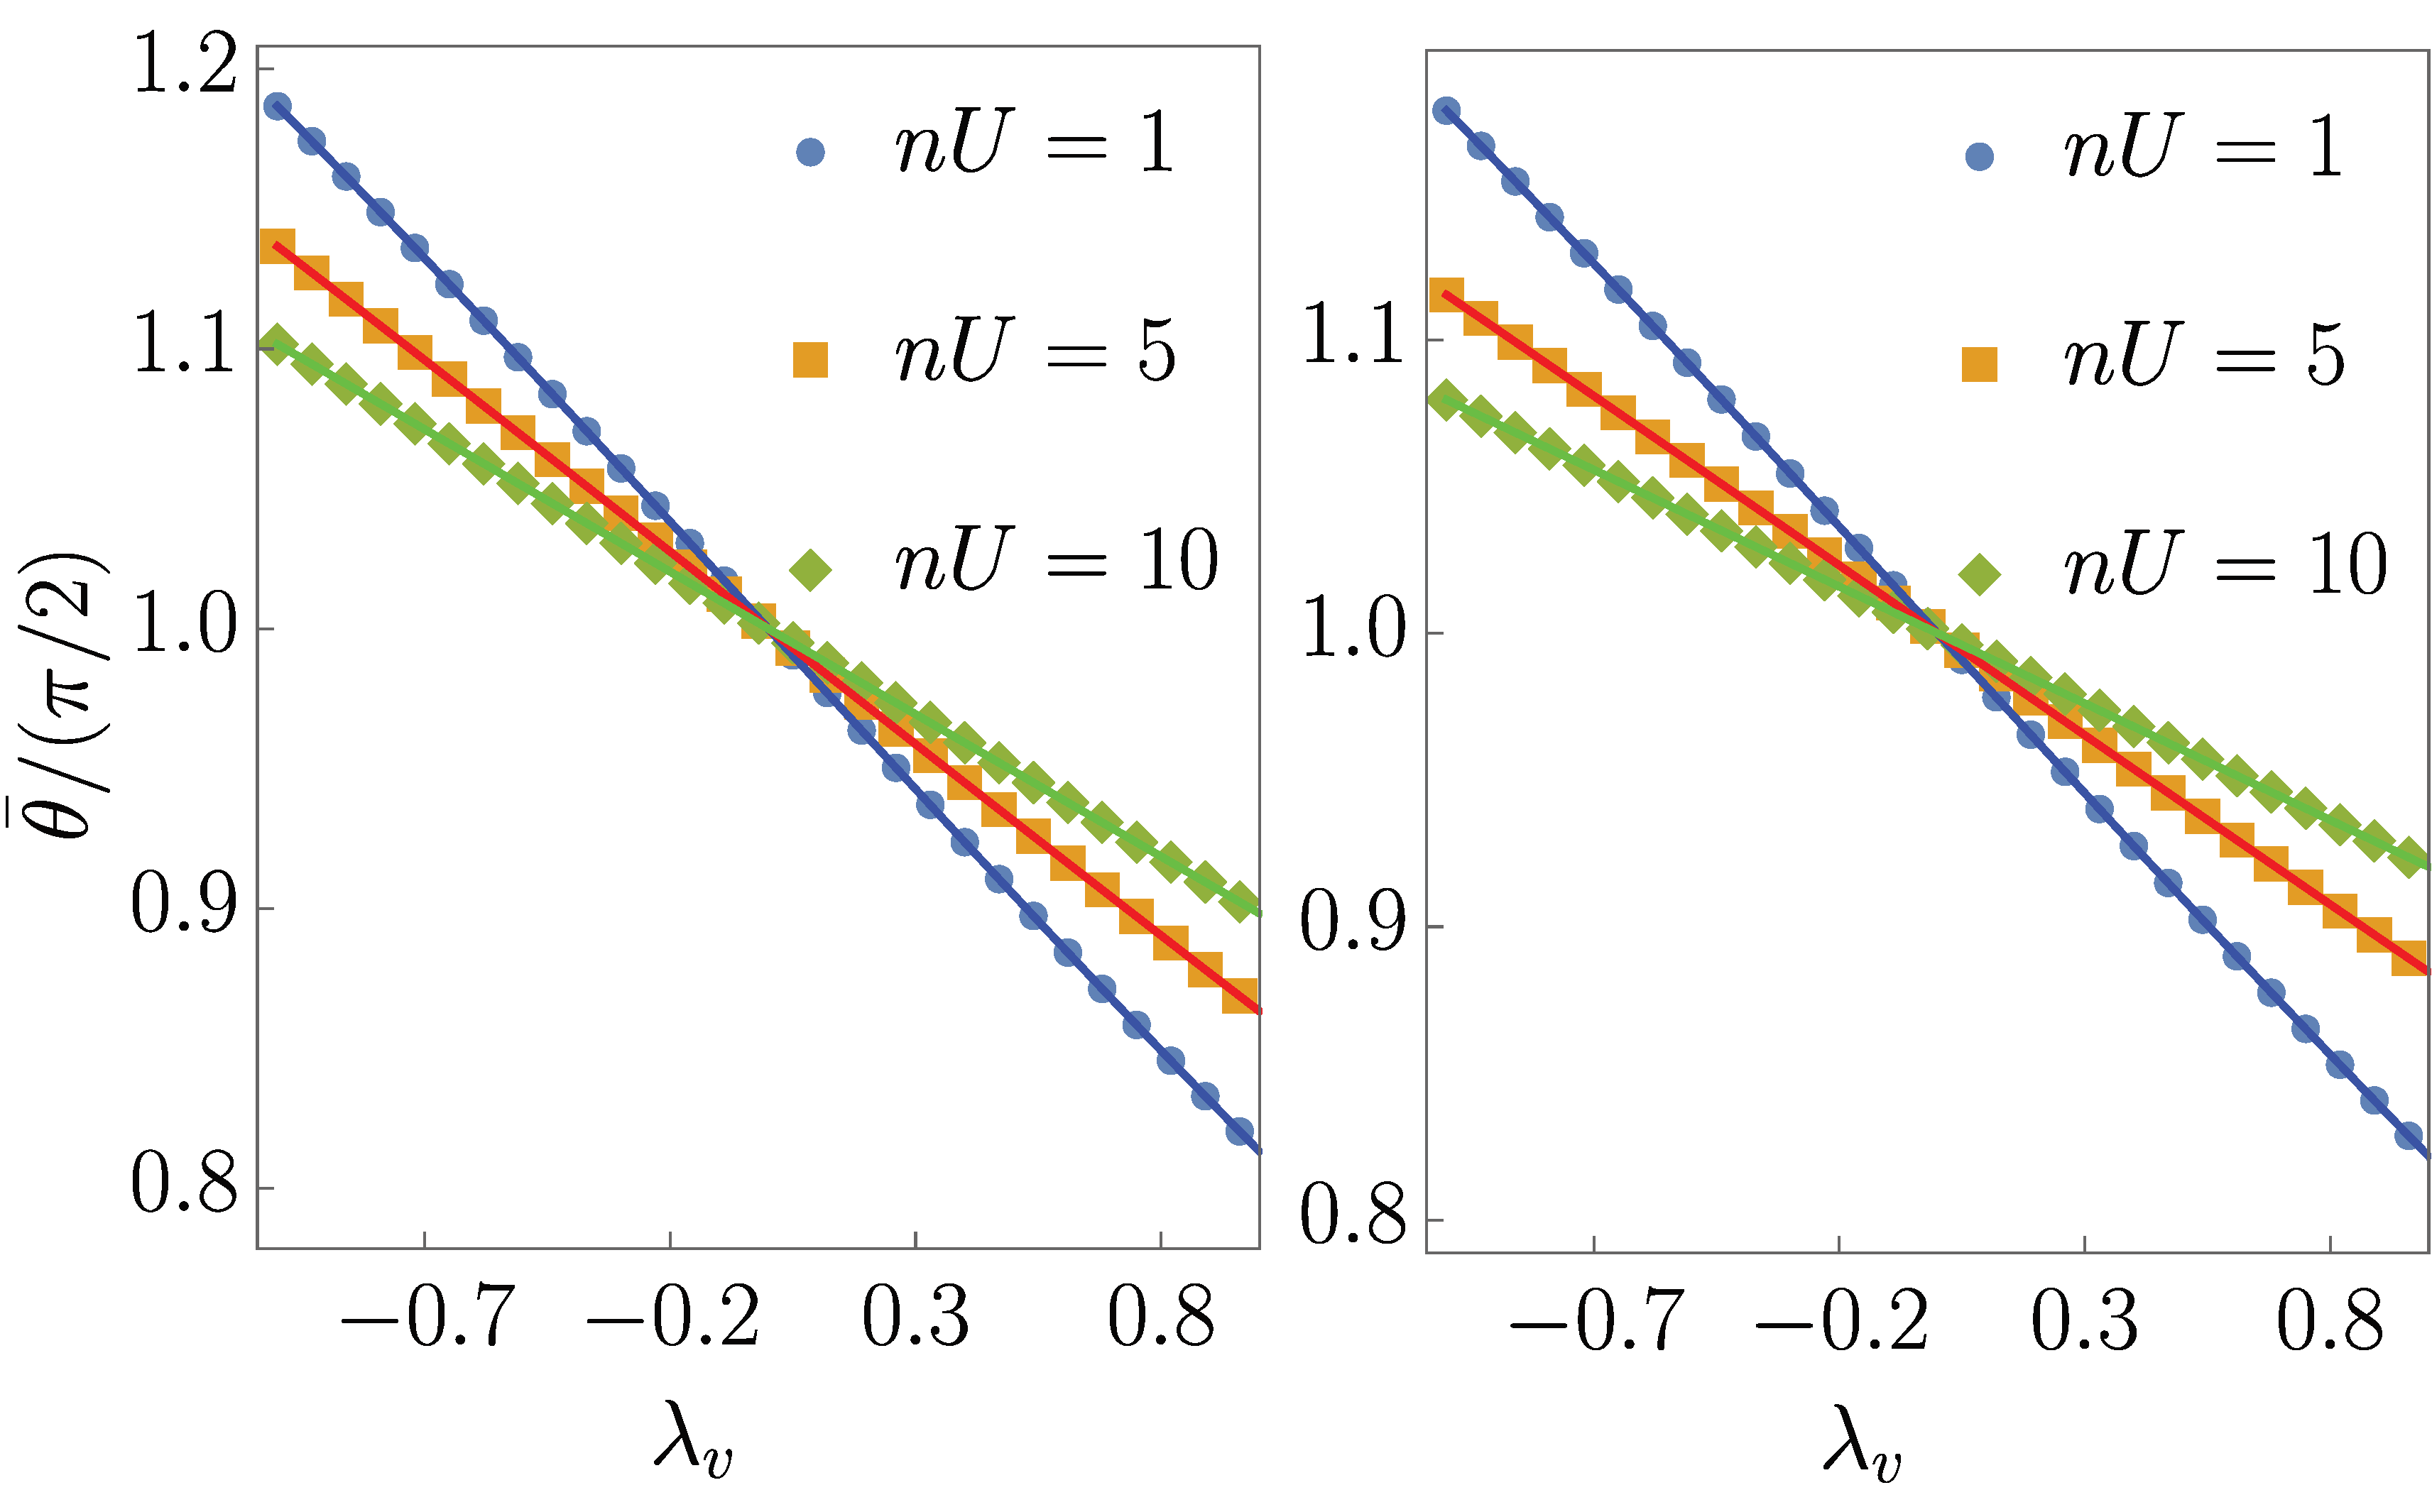
\includegraphics[width=.95\textwidth]{FIGthetabar.pdf}
	\caption{KMBH模型的平均场解,$\theta=2\arctan(\rho_3/\rho_1)$,对于不同的子晶格失衡$\lambda_v$和相互作用强度乘粒子数密度$nU$。左(右)图是种间相互作用各向异性$\lambda>0$($\lambda>0$)。
	离散点来自利用模拟退火数值最小化式\eqref{hmf}。实线来自最小化式\eqref{egp}和式\eqref{egp1}。
	注意虽然$\bar\theta$对于$\lambda>1$和$\lambda<1$有相似行为,
	系统基态一个处在Z顺磁态一个处在XY顺磁态。}
	\label{KMBHtheta}
\end{figure}
上述平均场的结果表明随着一个正的(负的)子晶格势被开启,$\bar \theta$从$\pi/2$开始减小(增大),
这个物理上就是指更多的玻色子会凝聚到$A$($B$)子晶格。
另一方面,排斥相互作用会压制这个子晶格的失衡,
因为前者更喜欢一个均匀的构型。
最后我们注意到$\bar \theta$是一个关于$\lambda_v$单调递减的函数,
但是对任意有限$\abs{\lambda_v}$,
它一直没达到极值$0$或者$\pi$。
这点与后面要讨论的BHZBH模型不同。

得到基态之后,我们根据粒子数守恒方案来计算Bogoliubov理论\cite{Kawaguchi2012}。
通过一下替换
\begin{equation}
	a^{(\dagger)}_{\boldsymbol{\Gamma}\sigma s} \rightarrow  \pqty{\mathcal N-\sum_{\vb k\neq\boldsymbol{\Gamma},\sigma s}a^\dagger_{\vb k,\sigma s}a_{\vb k,\sigma s}}^{1/2}\psi^{(*)}_{\sigma s},\nonumber
\end{equation}
最高到算符的二阶为止,式\eqref{KMBHfullh}变成
\begin{equation}\label{hbog}
	H_{\bog}=\mathcal N\mathcal E_\tgp + \sum_{\vb k\neq \boldsymbol{\Gamma}} a^\dagger_{\vb k}A_{\vb k} a_{\vb k} + (a^\dagger_{\vb k} B a^\dagger_{\vb k}+\hc),
\end{equation}
这里
\begin{align}
	A_{\vb k} & = h(\vb k) - \mu I_4 + h_1,\\
	\mu & = \sum_{\sigma s,\sigma' s'} \psi_{\sigma s}^* [h(\vb k)]_{\sigma s,\sigma' s'} \psi_{\sigma' s'},\\
	&\quad + n\sum_{\sigma s s'}U_{ss'}\psi^*_{\sigma s}\psi_{\sigma s'}^*\psi_{\sigma s'}\psi_{\sigma s},\\
	[h_1]_{\sigma s,\sigma' s'} & = n\delta_{\sigma,\sigma'}U_{s s'}(\psi_{\sigma s} \psi^*_{\sigma s'}+\psi^*_{\sigma s'}\psi_{\sigma s'}),
\end{align}
和
\begin{align}
	B_{\sigma s,\sigma' s'} = \frac{n}{2}\delta_{\sigma,\sigma'} U_{ss'} \psi_{\sigma s'}\psi_{\sigma s}.
\end{align}
我们把平均场结果带入式\eqref{hbog},
然后把它写成BdG形式。
对于$1>\lambda>0$,
有效哈密顿量是
\begin{equation}\label{KMBHheefl1}
	\begin{split}
	H^\eff_{\vb k}\vert_{\lambda<1} &= H^\eff_{\vb k}\vert_{\lambda=0} + \frac{\lambda nU}{8}\bigg\{i\tau_2\otimes(\cos\bar\theta \Gamma_{13}+\Gamma_{45})\\
	&\quad + \tau_3\otimes \big[\frac{\sin^2\bar\theta}{2} \Gamma_0 + \cos\bar\theta (\Gamma_2 + \Gamma_{13}) +\Gamma_{45}\big]\bigg\},
	\end{split}
\end{equation}
对于赝时间反演对称算符式\eqref{PTRSop1},
$\Gamma_{13}$和$\Gamma_{45}$到出现导致了赝时间反演对称性的缺失,对于任意的$1>\lambda>0$。
同时,对于$\lambda>1$,
有效哈密顿量是
\begin{equation}\label{KMBHheefg1}
	H^\eff_{\vb k}\vert_{\lambda>1} = H^\eff_{\vb k}\vert_{\lambda=0} + \frac{\lambda n U}{4}\tau_3\otimes \big[ \Gamma_0 + \cos\bar\theta (\Gamma_2 - \Gamma_{15}) - \Gamma_{34} \big].
\end{equation}
由于$\Gamma_{15}$和$\Gamma_{34}$的出现,我们同样没有赝时间反演对称性了。
在图\ref{KMBHwithoutPTRS}%
\begin{figure}
	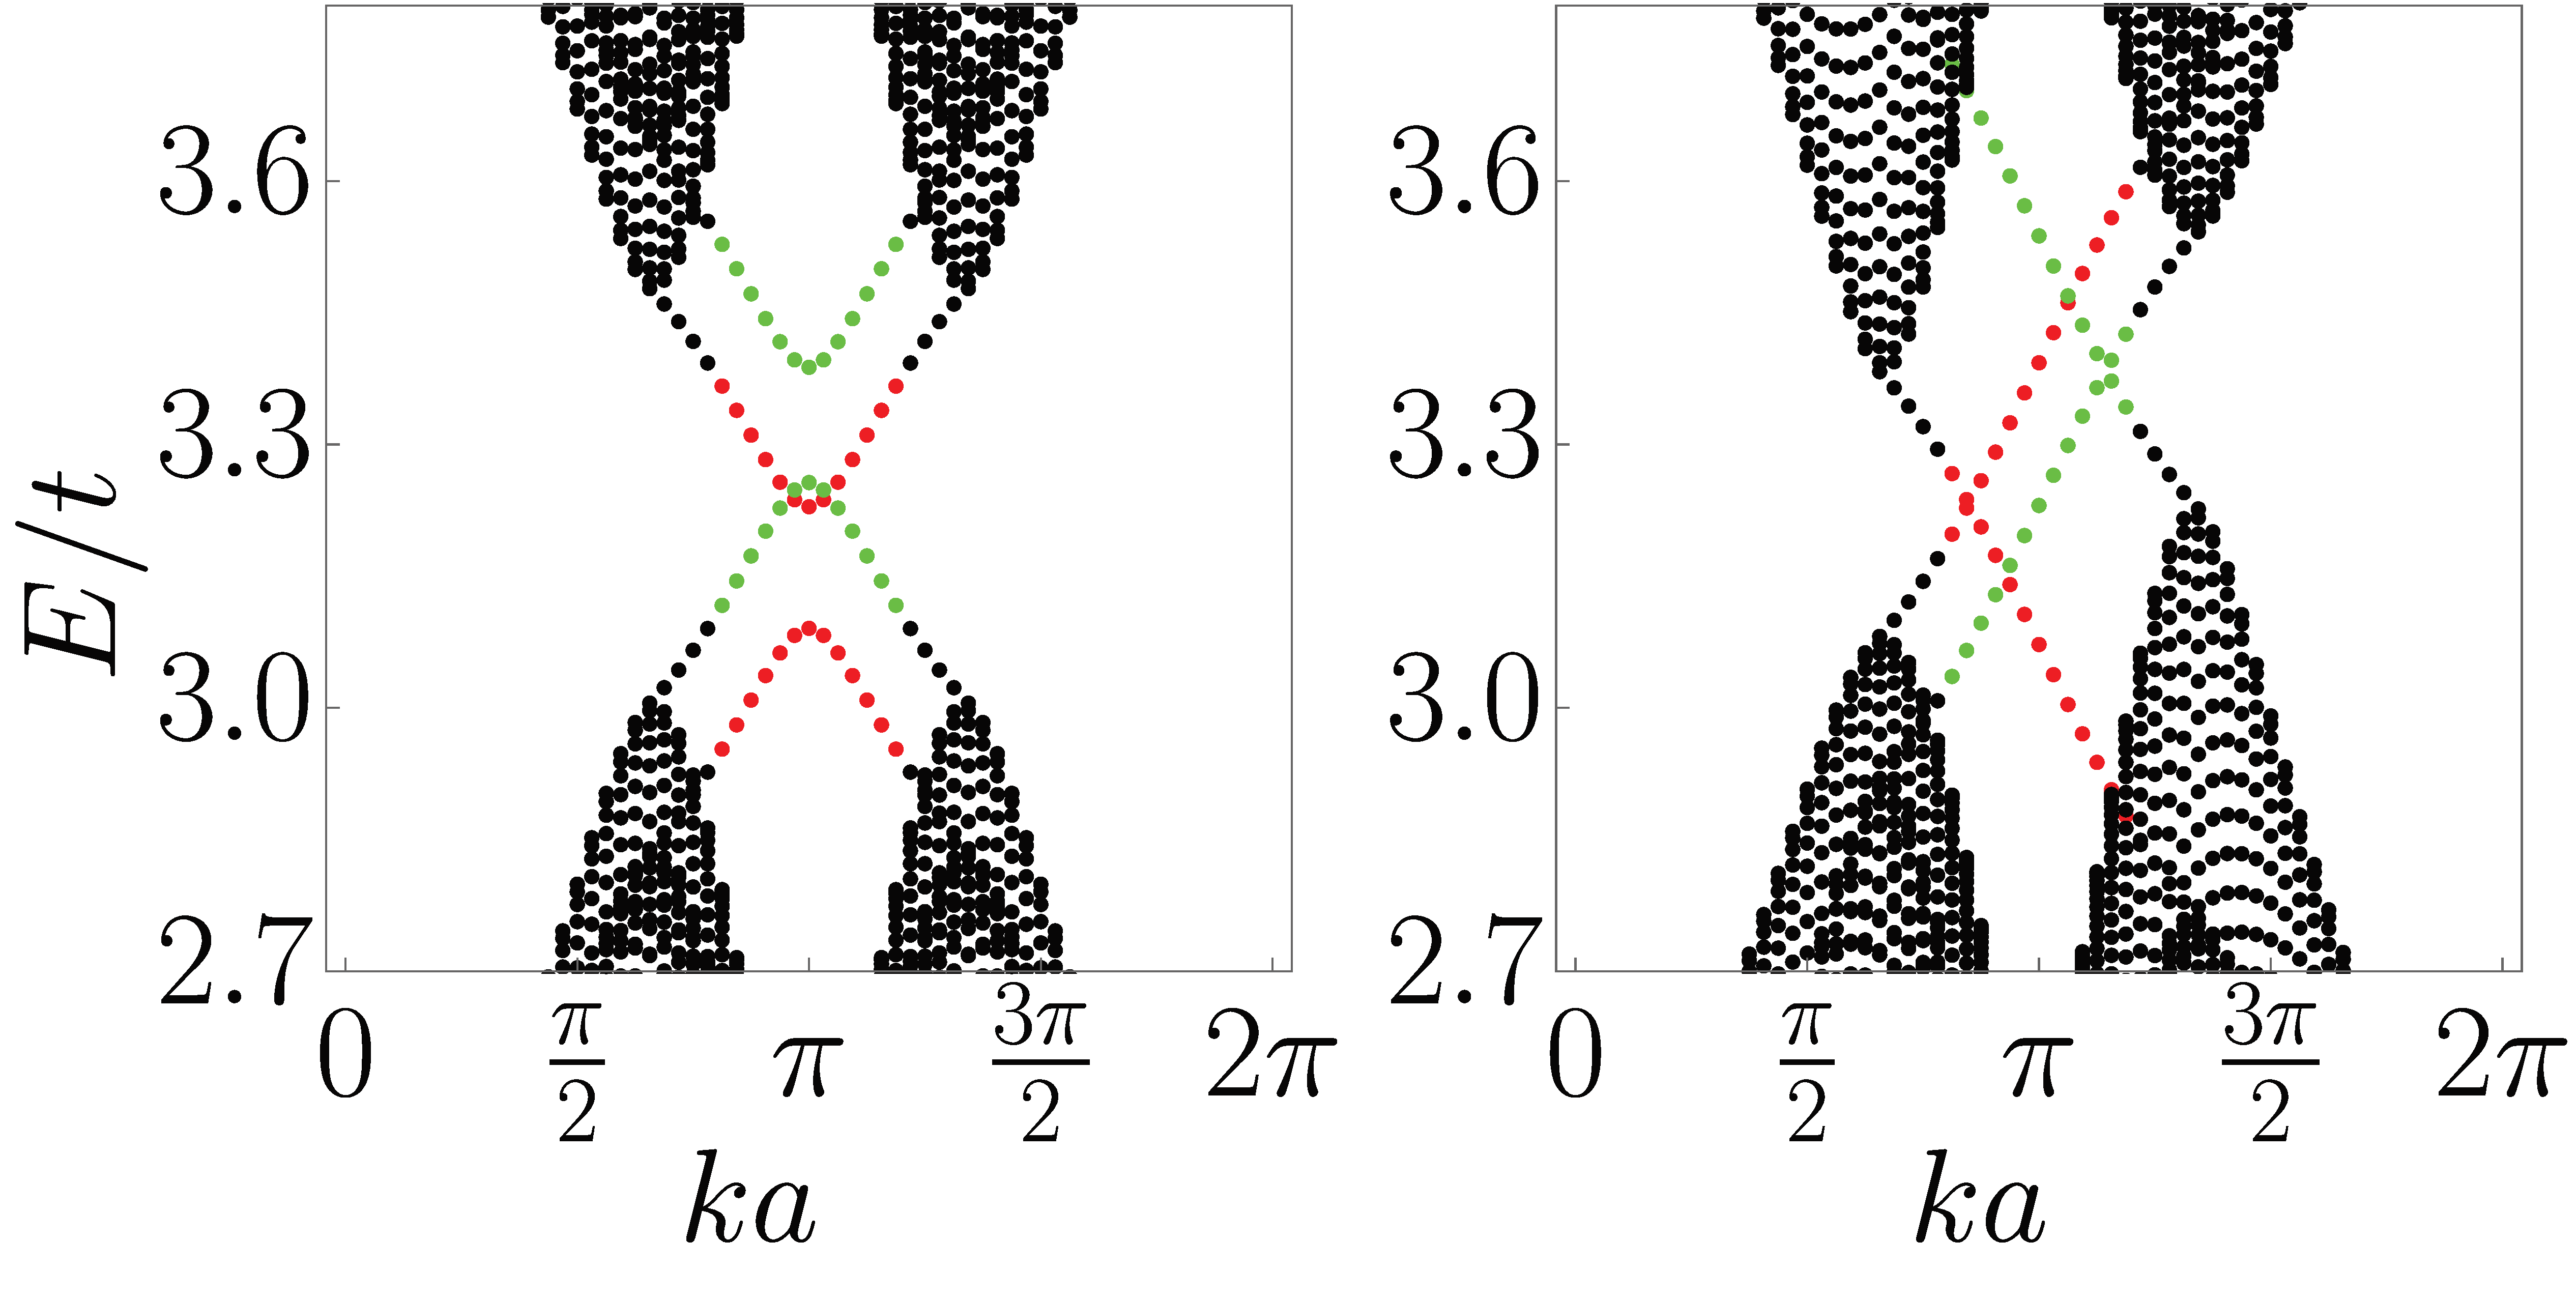
\includegraphics[width=.95\textwidth]{FIGbkmwithoutPTRS.pdf}
	\caption{对于在一个带状几何上的KMBH模型的Bogoliubov激发谱,这里一共有$64$晶胞(每个包含$64$个各点),用的zigzag边界,
	左边对应$\lambda=0.3$,右边对应$\lambda=1.3$。
	红/蓝点代表边界态,
	它们的波函数有大于$80\%$权重在最左/右的晶胞。
	显然这里已经没有玻色型的Kramers对。
	其他参数:$nU/t=1$,$\lambda_s/t=0.06$和$\lambda_v/t=0.1$。}
	\label{KMBHwithoutPTRS}
\end{figure}
我们展示了对于$0<\lambda<1$和$\lambda>1$,这里没有玻色型的Kramers对。
总而言之,种间相互作用将会破坏赝时间反演对称性。







\subsection{BHZBH模型}
BHZBH模型在k空间的带有一般排斥相互作用的完整哈密顿量是
\begin{equation}\label{BHZBHfullh}
\begin{split}
	&H = \sum_{\vb k}a^\dagger_{\vb k}h(\vb k)a_{\vb k} + \frac{1}{2M}\\
	&\times \sum_{\vb k,\vb p,\vb q,\eta\eta' s s'} U_{\eta s,\eta's'}a^\dagger_{\vb k+\vb q,\eta s}a^\dagger_{\vb p-\vb q,\eta' s'}a_{\vb k,\eta' s'}a_{\vb p,\eta s},
\end{split}
\end{equation}
这里$h(\vb k)$由式\eqref{hkbhz}给出。
为了简化讨论,
我们假设如果$\eta=\eta'$和$s=s'$,$U_{\eta s,\eta' s'}=U$,其他情况下$U_{\eta s,\eta' s'}=\lambda U$。
物理上,我们考虑在位的,
所有四类玻色子之间的密度-密度相互作用。注意这与KMBH不同,后者只有两类玻色子。
假设玻色子凝聚在$\boldsymbol{\Gamma}$,
只要$m_z$足够大,这个总是可以的。
那么基态波函数ansatz是
\begin{equation}
	\ket{\psi}=\frac{1}{\sqrt{\mathcal N!}}\pqty{\sqrt{\mathcal N}\sum_{\eta s}\psi_{\eta s}a_{\boldsymbol{\Gamma}\eta s}^\dagger}^{\mathcal N}\ket{0},\nonumber
\end{equation}
其中四个复数满足$\sum_{s}\abs{\psi_{\eta s}}^2=1$。
利用式\eqref{parametrization},
GP能量泛函变成\footnote{注意GP能量泛函是独立于所有相位因子$\phi_i$,$i=1,\dots,4$的,这是由于存在两个严格的U(1)对称性,以及偶然对称性。后者可以通过考虑量子涨落解除,例如,\cite{You2012}。}
\begin{equation}\label{egpBHZBH}
	\begin{split}
		\mathcal E_\tgp &= -(4t+m_z)(\rho_1^2-\rho_2^2+\rho_3^2-\rho_4^2)\\
		&\quad + nU\bigg[\frac{1}{2}+(\lambda-1) (\rho_1^2\rho_2^2 +\rho_1^2\rho_3^2\\
		&\quad + \rho_1^2\rho_4^2 + \rho_2^2\rho_3^2 +\rho_2^2\rho_4^2 + \rho_3^2\rho_4^2)\bigg].
	\end{split}
\end{equation}
对于$0\leq\lambda<1$,通过令$\rho_1=\rho_3=(1/\sqrt{2})\cos\frac{\bar\theta}{2}$和$\rho_2=\rho_4=(1/\sqrt{2})\sin\frac{\bar\theta}{2}$,其中$\bar\theta$在图\ref{BHZBHtheta}%
\begin{figure}
	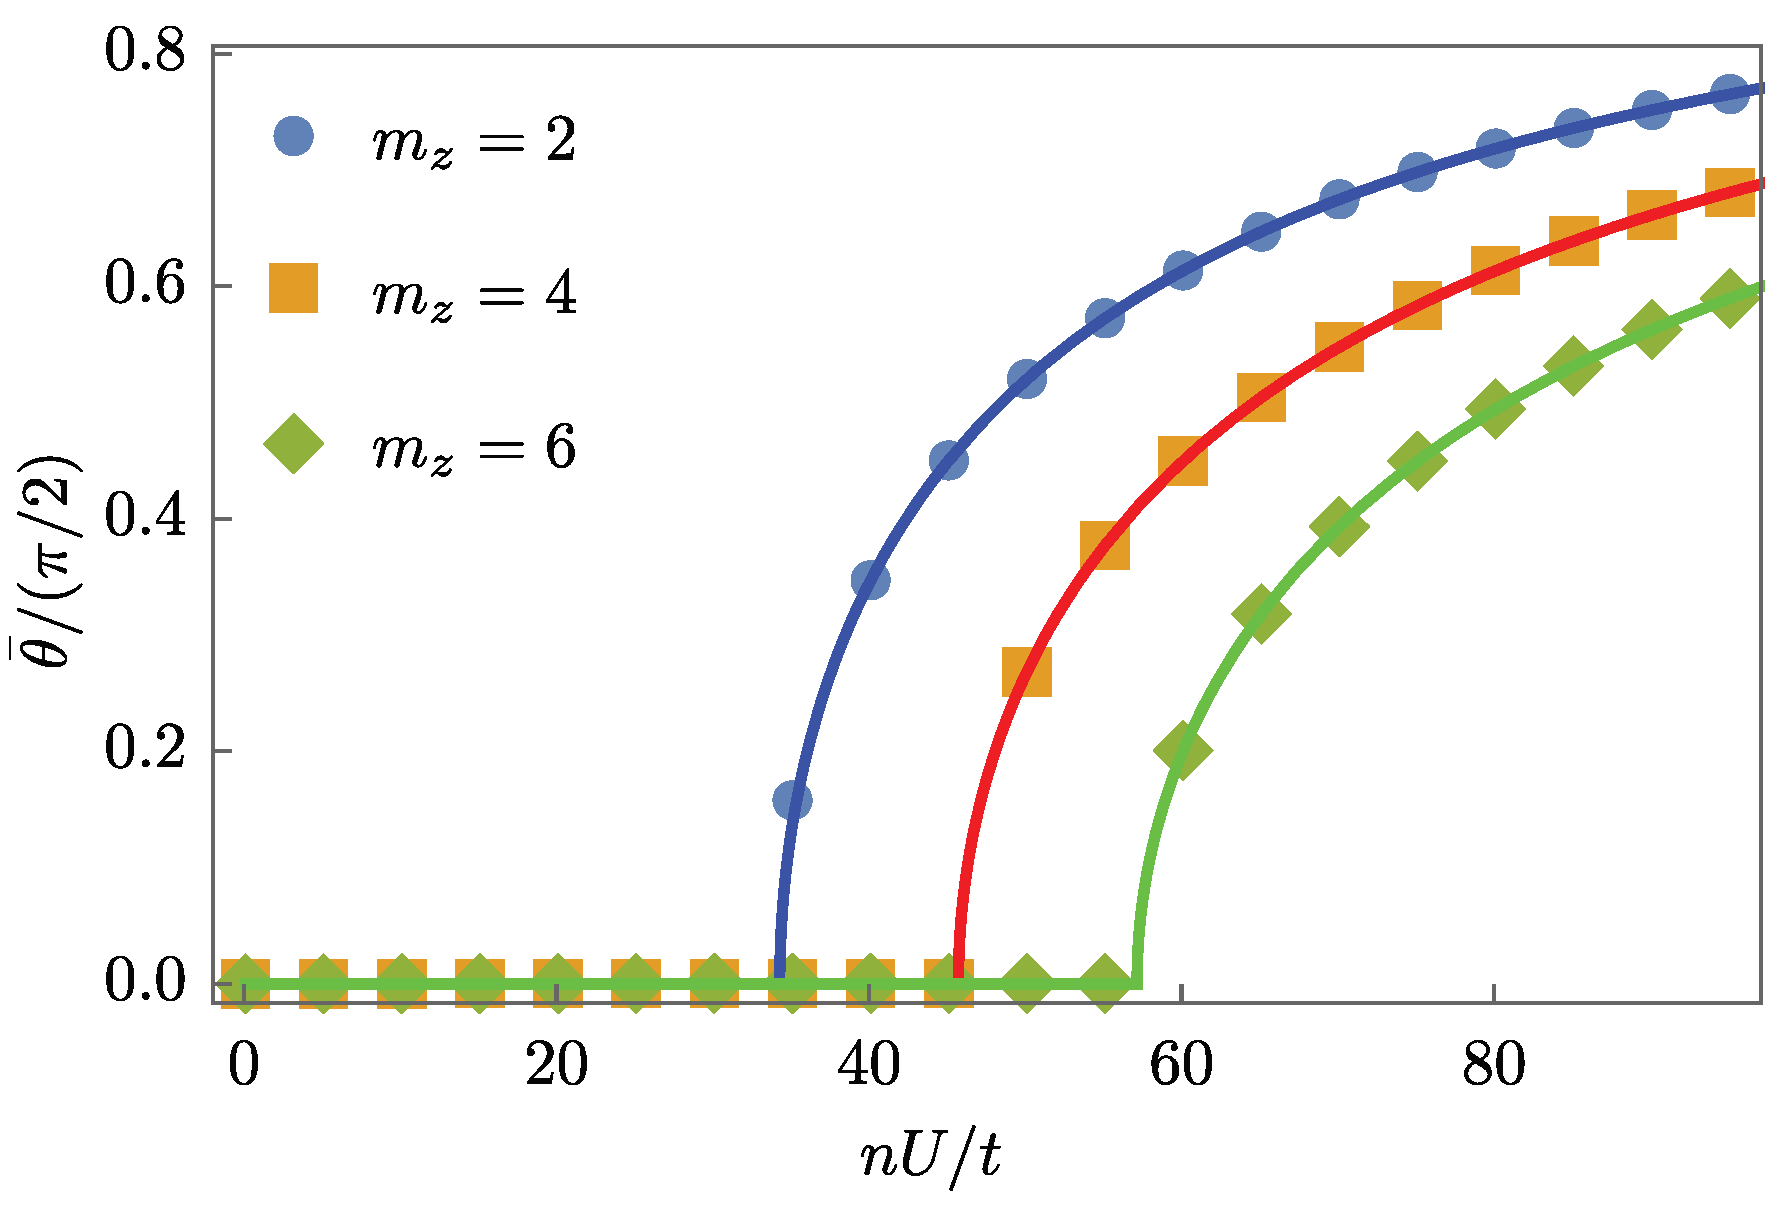
\includegraphics[width=.95\textwidth]{FIGthetabar1.pdf}
	\caption{对于BHZBH模型的平均场解$\theta=2\arctan(\rho_2/\rho_1)$,作为$nU$和$m_z$的函数,这里$\lambda=0.3$。注意当在弱耦合区间,即$U/t$很小,我们总有$\bar\theta=0$。}
	\label{BHZBHtheta}
\end{figure}
给出,式\eqref{egpBHZBH}可以被最小化。
注意对于弱耦合极限,即$U/t$很小,
我们总有$\bar\theta=0$,
以下我们假设这个条件成立。
对于$\lambda>1$,
通过令$\rho_1=1$和$\rho_2=\rho_3=\rho_4=0$
(或者由于对称性,交换$\rho_1$和$\rho_3$)
式\eqref{egpBHZBH}可以被最小化。

利用上面得到的平均场基态,我们可以计算Bogoliubov理论,通过把以下替换带入式\eqref{BHZBHfullh},
\begin{equation}
	a^{(\dagger)}_{\boldsymbol{\Gamma}\eta s} \rightarrow  \pqty{\mathcal N-\sum_{\vb k\neq\boldsymbol{\Gamma},\eta s}a^\dagger_{\vb k,\eta s}a_{\vb k,\eta s}}^{1/2}\psi^{(*)}_{\eta s}.\nonumber
\end{equation}
到二阶为止,Bogoliubov哈密顿量有和式\eqref{hbog}一样的形式,
其中$\mathcal E_\tgp$由式\eqref{egpBHZBH}给出,
$A,B$如下
\begin{align}
	A_{\vb k} &= h(\vb k) - \mu I_4 + h_1 \\
	\mu &= \sum_{\eta s,\eta' s'}\psi^*_{\eta s}[h(\vb k)]_{\eta s,\eta' s'}\psi_{\eta' s'}\\
	&\quad +n\sum_{\eta s,\eta' s'} U_{\eta s,\eta' s'} \psi^*_{\eta s} \psi^*_{\eta' s'}\psi_{\eta' s'}\psi_{\eta s} \\
	[h_1]_{\eta s,\eta' s'} &= n  U_{\eta s,\eta' s'}(\psi_{\eta s}\psi^*_{\eta's'}+\psi_{\eta' s'}^*\psi_{\eta' s'})
\end{align}
和
\begin{equation}
	B_{\eta s,\eta' s'}=\frac{n}{2} U_{\eta s,\eta' s'} \psi_{\eta' s'}\psi_{\eta s}.
\end{equation}
把平均场基态解带入式\eqref{BHZBHfullh},
对于$1>\lambda>0$,
有效哈密顿量是
\begin{equation}
	\begin{split}
		H^\eff_{\vb k} \vert_{\lambda<1} &= H^\eff_{\vb k}\vert_{\lambda=0} + \frac{\lambda nU}{4}   \tau_3\otimes (-\Gamma_{23}+\Gamma_{45}+3\Gamma_0-\Gamma_1)\\
	&\quad +\frac{\lambda nU}{4} i   \tau_2 \otimes (-\Gamma_{23}+\Gamma_{45})
	\end{split}
\end{equation}
对于定义在式\eqref{PTRSop2}中的赝时间反演对称算法,
我们有(对于定义在式\eqref{ISop}中的$\mathcal P$,下面右边的的加号和减号互换即可)
\begin{equation}
	\mathcal T [\tau_i \otimes \Gamma_{ab}] \mathcal T = \begin{cases}
		&+\tau_i \otimes\Gamma_{ab} \qfor a=1 \qor b=1,\\
		&-\tau_i \otimes\Gamma_{ab} \qfor a \neq 1 \qand b \neq 1.
	\end{cases}\nonumber
\end{equation}
所以对于$1>\lambda>0$,$\Gamma_{23}$和$\Gamma_{45}$的出现导致这个BdG系统没有赝时间反演对称性,
但仍有空间反演对称。
对于$\lambda>1$,
有效哈密顿量是
\begin{equation}
	H^\eff_{\vb k}\vert_{\lambda>1} = H^\eff_{\vb k}\vert_{\lambda=0}+\frac{\lambda nU}{4}\tau_3\otimes (-\Gamma_{34}+\Gamma_{25}+3\Gamma_0-\Gamma_1)
\end{equation}
同样的,$\Gamma_{34}$和$\Gamma_{25}$的出现导致赝时间反演对称性的缺失,但仍有空间反演对称性。
图\ref{BHZBHwithoutPTRS}%
\begin{figure}
	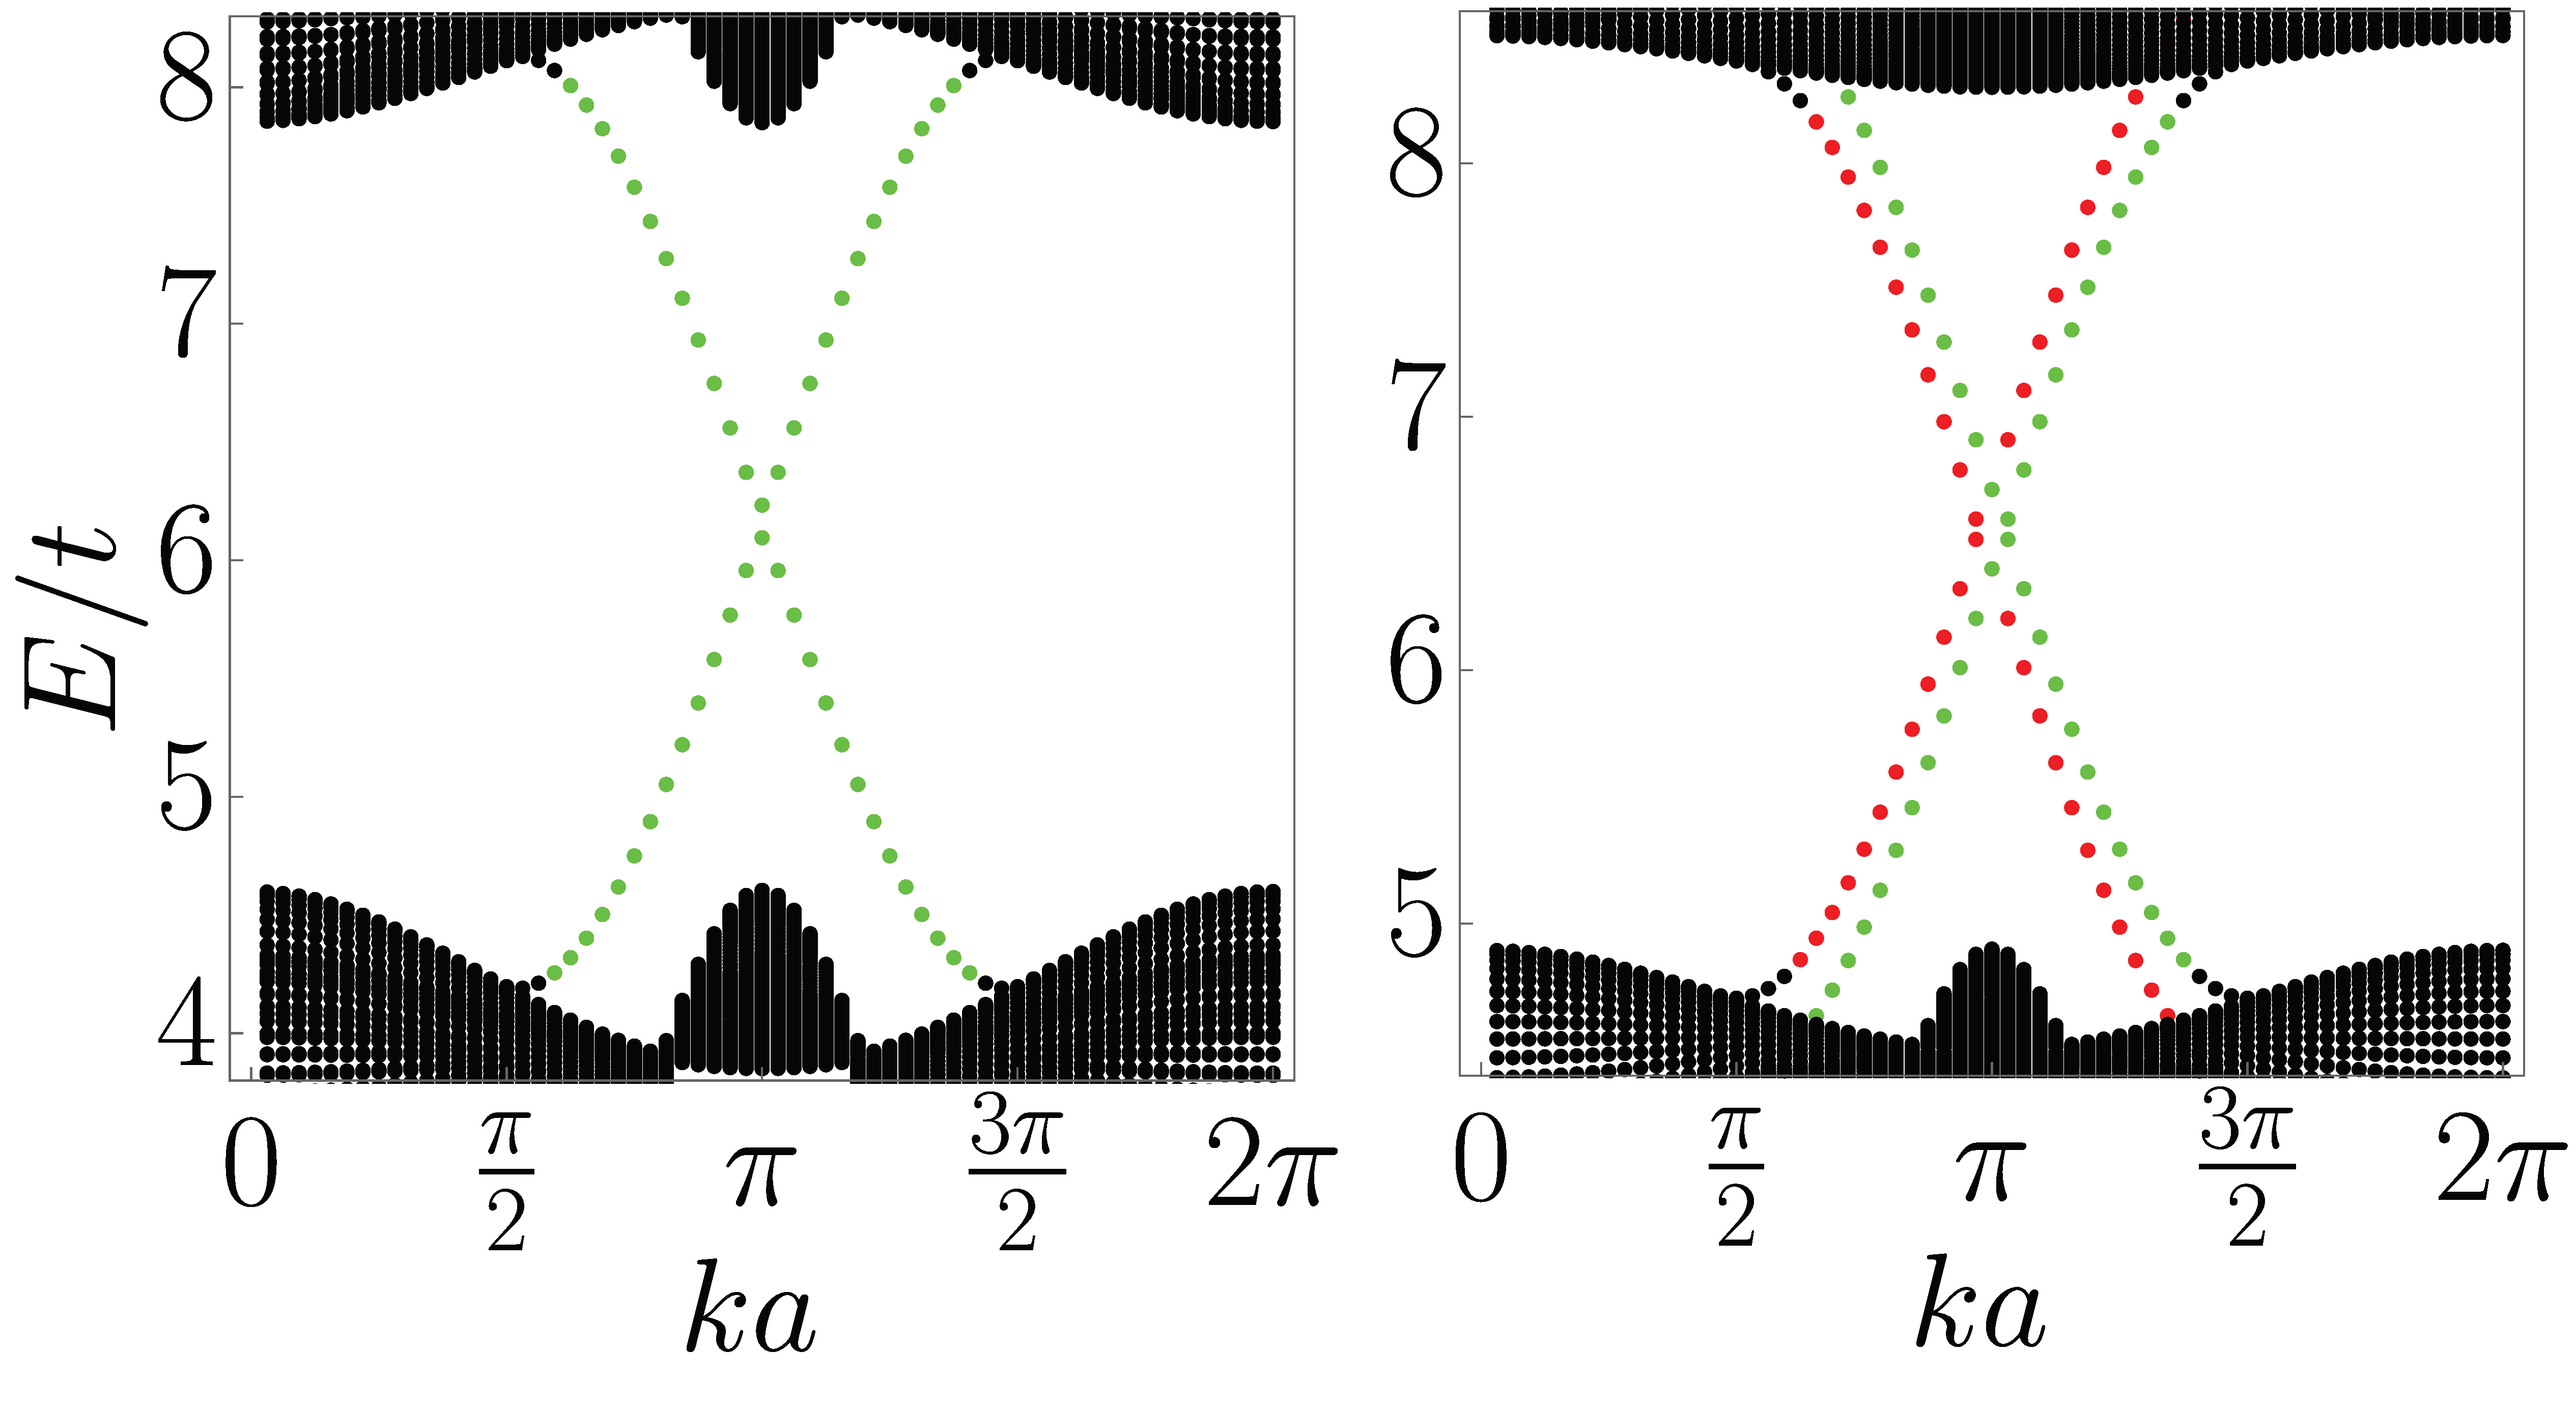
\includegraphics[width=.95\textwidth]{FIGbbhzwithoutPTRS.pdf}
	\caption{对于$\lambda=0.3$(左)和$\lambda=1.3$(右),BHZBH模型在一个带状几何上的Bogoliubov激发谱。这里我们考虑有$64$个晶胞。其中红/蓝点表示边界态,对应于波函数有大于$80\%$的比例在最左/右边的晶胞。注意对于左图,两种边界态由于空间反演对称性完全重合了。可以看见,这里没有玻色型的Kramers对。其他参数:$nU/t=t_s/t=1$和$m_z/t=2.1$。}
	\label{BHZBHwithoutPTRS}
\end{figure}
展示了,对于$0<\lambda<1$和$\lambda>1$,玻色型Kramers对是不存在的。
总而言之,这里种间相互作用同意会破坏赝时间反演对称性。








